\documentclass{beamer}
\usepackage{graphicx}
\graphicspath{ {./images/} }
\usepackage[rightcaption]{sidecap}

\usefonttheme[onlymath]{serif}
\definecolor{LHCblue}{RGB} {180,199,231}%{4, 114, 255}
\usecolortheme[named=LHCblue]{structure}
\usepackage[bars]{beamerthemetree} % Beamer theme v 2.2
\usepackage{multicol}
\usepackage{lmodern}
\usepackage{lipsum}
\usepackage{marvosym}

\usetheme{Berlin}
\setbeamertemplate{blocks}[default]
\useinnertheme{circles} % change the bullets' shape
\setbeamertemplate{caption}[numbered] % number the figures
\usepackage[textfont={scriptsize}]{caption}
\usepackage{tikz} % for checkmarks
\setbeamertemplate{blocks}[rounded][shadow=true]

%\setbeamertemplate{footline}{\begin{tikzpicture}
%    \node [inner sep=0pt, anchor=east] (0,0) {
\includegraphics[width=\paperwidth,height=0.8cm]{15_footnote_all}};
%%    \node [inner sep=0pt, anchor=east] at (-2ex,-3ex) {\insertframenumber{} / %\inserttotalframenumber};
%\end{tikzpicture}}

\title{Open tools and methodology for the development of a web-based transportation platform}
%\author{Babalis B*, Ballis A., Koukoutsis E.}
%\institute{National Technical University of Athens}
%\date{2021}

\author[Babalis B., Ballis A., Koukoutsis E.] % (optional, for multiple authors)
{Babalis B.\inst{1} \and Ballis A.\inst{2} \and Koukoutsis E.\inst{1}}

\institute[National Technical University of Athens] % (optional)
{
  \inst{1}%
  School of Electrical and Computer Engineering\\
  National Technical University of Athens
  \and
  \inst{2}%
  School of Civil Engineering\\
  National Technical University of Athens
}

\date[CES 2021] % (optional)
{Circular Economy and Sustainability, July 2021}

% conditional for logo. \placelogofalse removes both enirisst and pyrforos
\newif\ifplacelogo % create a new conditional
\placelogotrue % set it to true
%\logo{
\includegraphics[height=1cm]{09_pyrforos_bw}}
\logo{\ifplacelogo
  
\includegraphics[width=1cm,height=1cm,keepaspectratio]{13_enirisst}%
  \hspace{\dimexpr\paperwidth-2cm-5pt}%
  
\includegraphics[width=1cm,height=1cm,keepaspectratio]{09_pyrforos_bw}%
\fi}
\usepackage{textpos}

\begin{document}

\frame{\titlepage}
%
%\begin{frame}
%	\frametitle{Table of Contents}
%	\tableofcontents
%\end{frame}

\section{Introduction}

	\begin{frame}
	\frametitle{Scope of the Presentation}
	\begin{itemize}
    	\item Describe a web-based transportation platform built with open data and tools.
    	\item Present the platform from functionality and usability perspective.
    \end{itemize}
	
	\end{frame}

    \begin{frame}
    \frametitle{Introduction}
    \emph{Transportation platform:} Supports all activities relating to transport, logistics and the distribution of goods.\\
    Usually transportation platforms offer functionality based on:
    \begin{itemize}
    	\item Proprietary GIS systems.
    	\item Proprietary updates on network and data.
    	\item External, proprietary web applications.
    \end{itemize}
    \pause
    \checkmark As a result, such platforms heavily depend on their proprietary software.
    \end{frame}
    
    \begin{frame}
    \frametitle{Alternative Approach: Open Data and Tools Platform}
    Platform based on free and open source data and tools.
    
    \begin{itemize}
        \item Open Data.
        \item Open source tools for building the platform.
        \item Open Maps.
    \end{itemize}
    \pause
    \begin{block}{Why open data andtools?}
    \begin{itemize}
        \item \textbf{Sustainability/Maintainability:} no dependencies on proprietary tools.
        \item \textbf{Reliability:} Maps data checked and maintained by the community.
    \end{itemize}
    \end{block}
    
    \end{frame}

\section{Architecture and Design}
    \begin{frame}
    \frametitle{Basic Platform Components}
    Basic blocks for building a web transportation platform:
    \begin{enumerate}
        \item Maps and geospatial data visualization tools.
        \item Data and tools for data selection and process.
        \item Set of functionalities offered through a web interface.
    \end{enumerate}
    
	\end{frame}
	
	\begin{frame}
    \frametitle{Abstract Methodology}
    For the alternative platform to be developed the following steps applied:
    
    \begin{itemize}
        \item Maps collected and integrated to the platform.
        \item Open Data collected.
        \item Data organized and integrated to the platform.
        \item Data visualizations offered (through charts/pies and maps).
        \item Extra functionalities developed combining the data collected with geospatial information.
    \end{itemize}
    
    \end{frame}
    
    \begin{frame}
    \frametitle{High-level Architecture of the Platform}
    \begin{figure}[h]
    \centering
    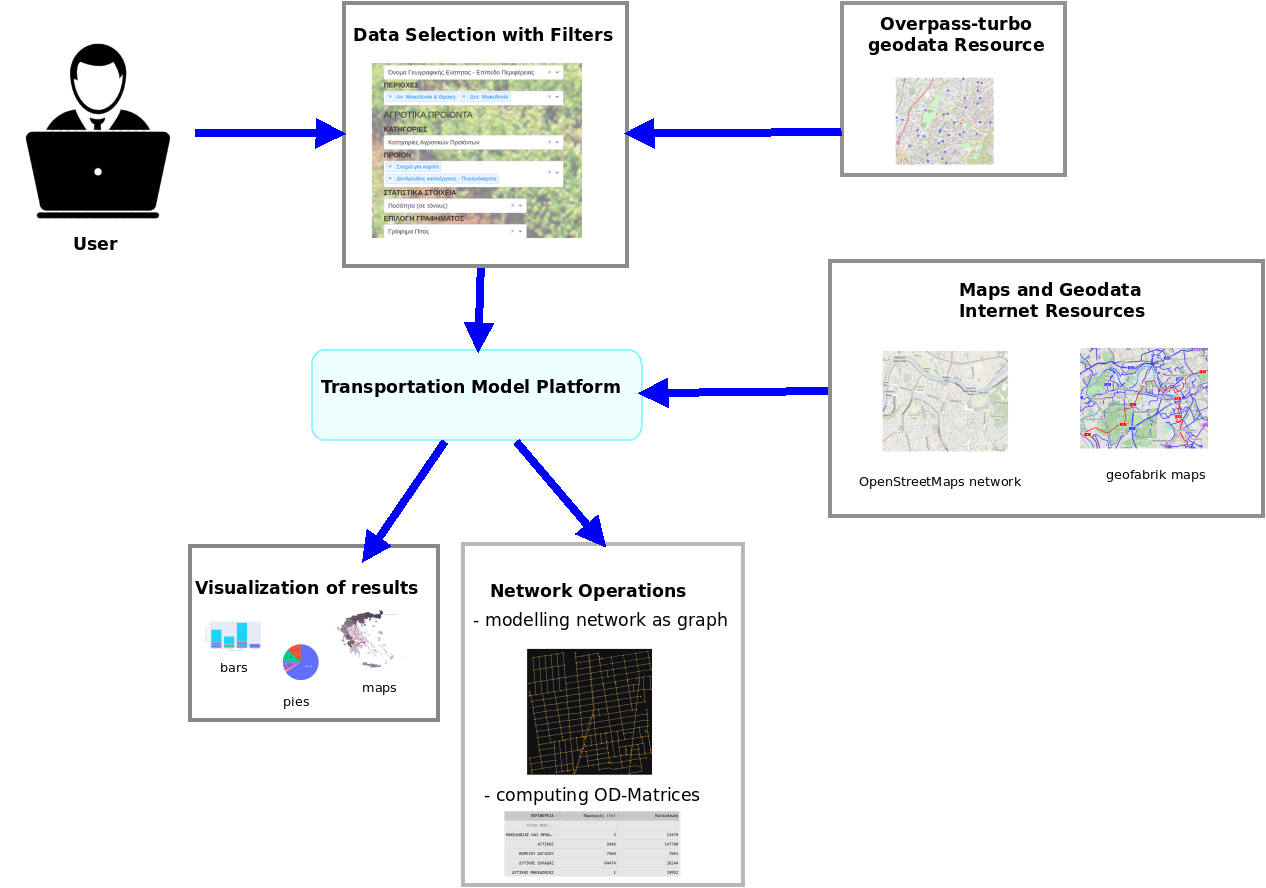
\includegraphics[width=8cm, height=5cm]{10_conceptual-architecture}
    \caption{Conceptual Architecture of the Platform.}
    \label{fig:arch}
    \end{figure}
    \end{frame}
    
   \section{Methodology}
    \begin{frame}
    \frametitle{Maps}
    The maps selected for the platform are the OpenStreetMaps (OSM).
    OSM is a collaborative project that creates a free, editable map of the world.
    
    \begin{block}{OpenStreetMaps}
		\begin{itemize}
        	\item It covers the world.
        	\item It is supported by OpenStreetMap Foundation (non-profit organization).
        	\item Open Database License (ODbL)
    	\end{itemize}
	\end{block}
    
    \end{frame}
    
    \begin{frame}
    \frametitle{Platform Data}
    
    \begin{itemize}
    	\item EN.I.R.I.S.S.T Service: “Transport \& Agrologistics” example.
        \item Data has been collected from elstat.
        \item Data has been normalized and filters may be applied to create a custom configuration.
    \end{itemize}
    
    \begin{figure}[h]
    \centering
    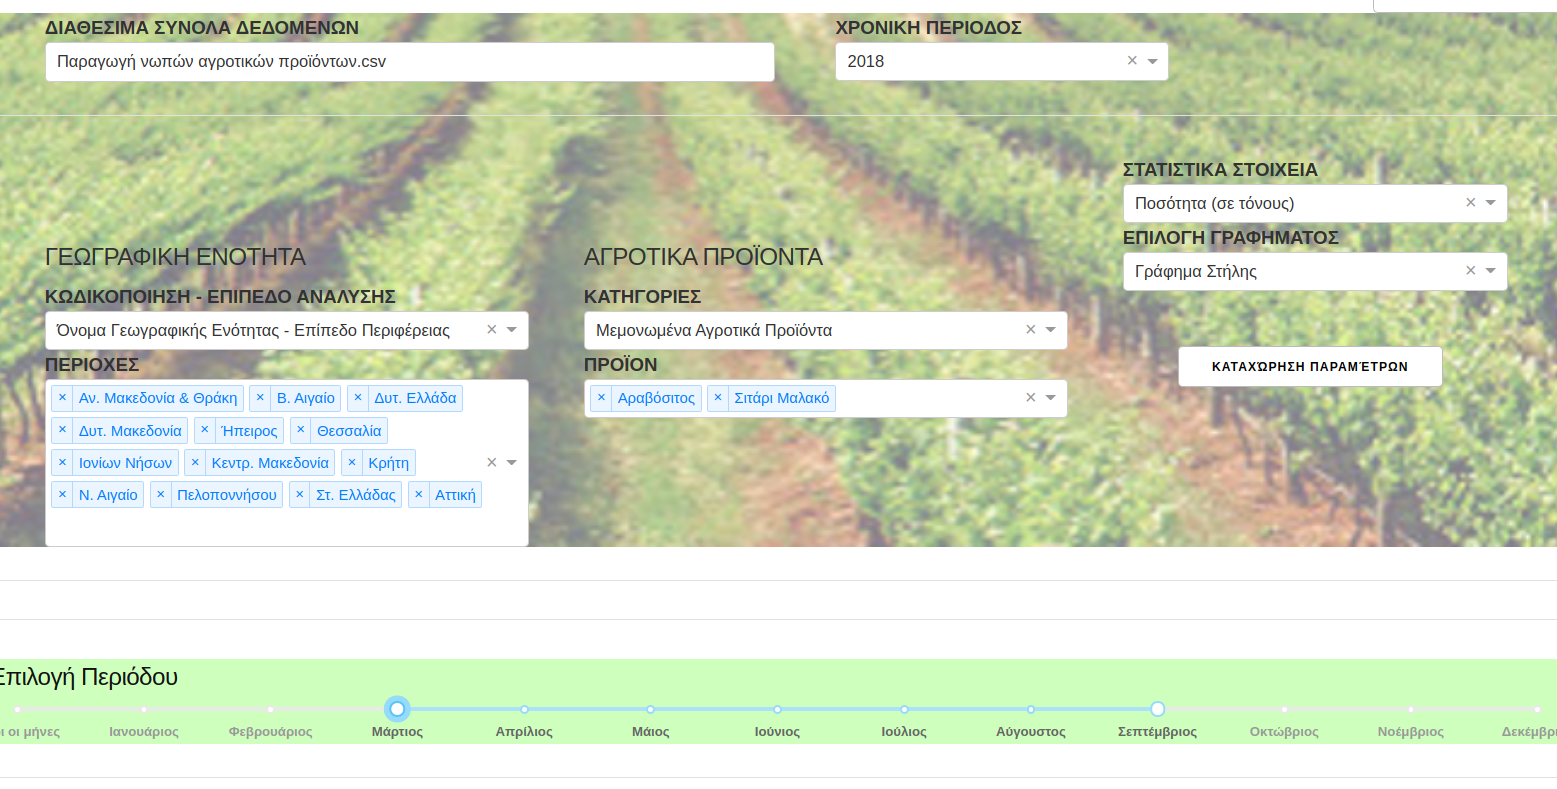
\includegraphics[width=7cm, height=3cm]{1_platform_filters}
    \caption{Filters applied to data available.}
    \label{fig:filters1}
    \end{figure}
    
    \end{frame}
    
    \begin{frame}
    \frametitle{Data Visualizations}
    
	    \begin{exampleblock}{Visualizing data}
	    Data selection is visualized through tables, charts, pies and choropleths.
		\end{exampleblock}
		
	%	\centering
	%        \begin{tabular}{c}
	%        example1\\
	%        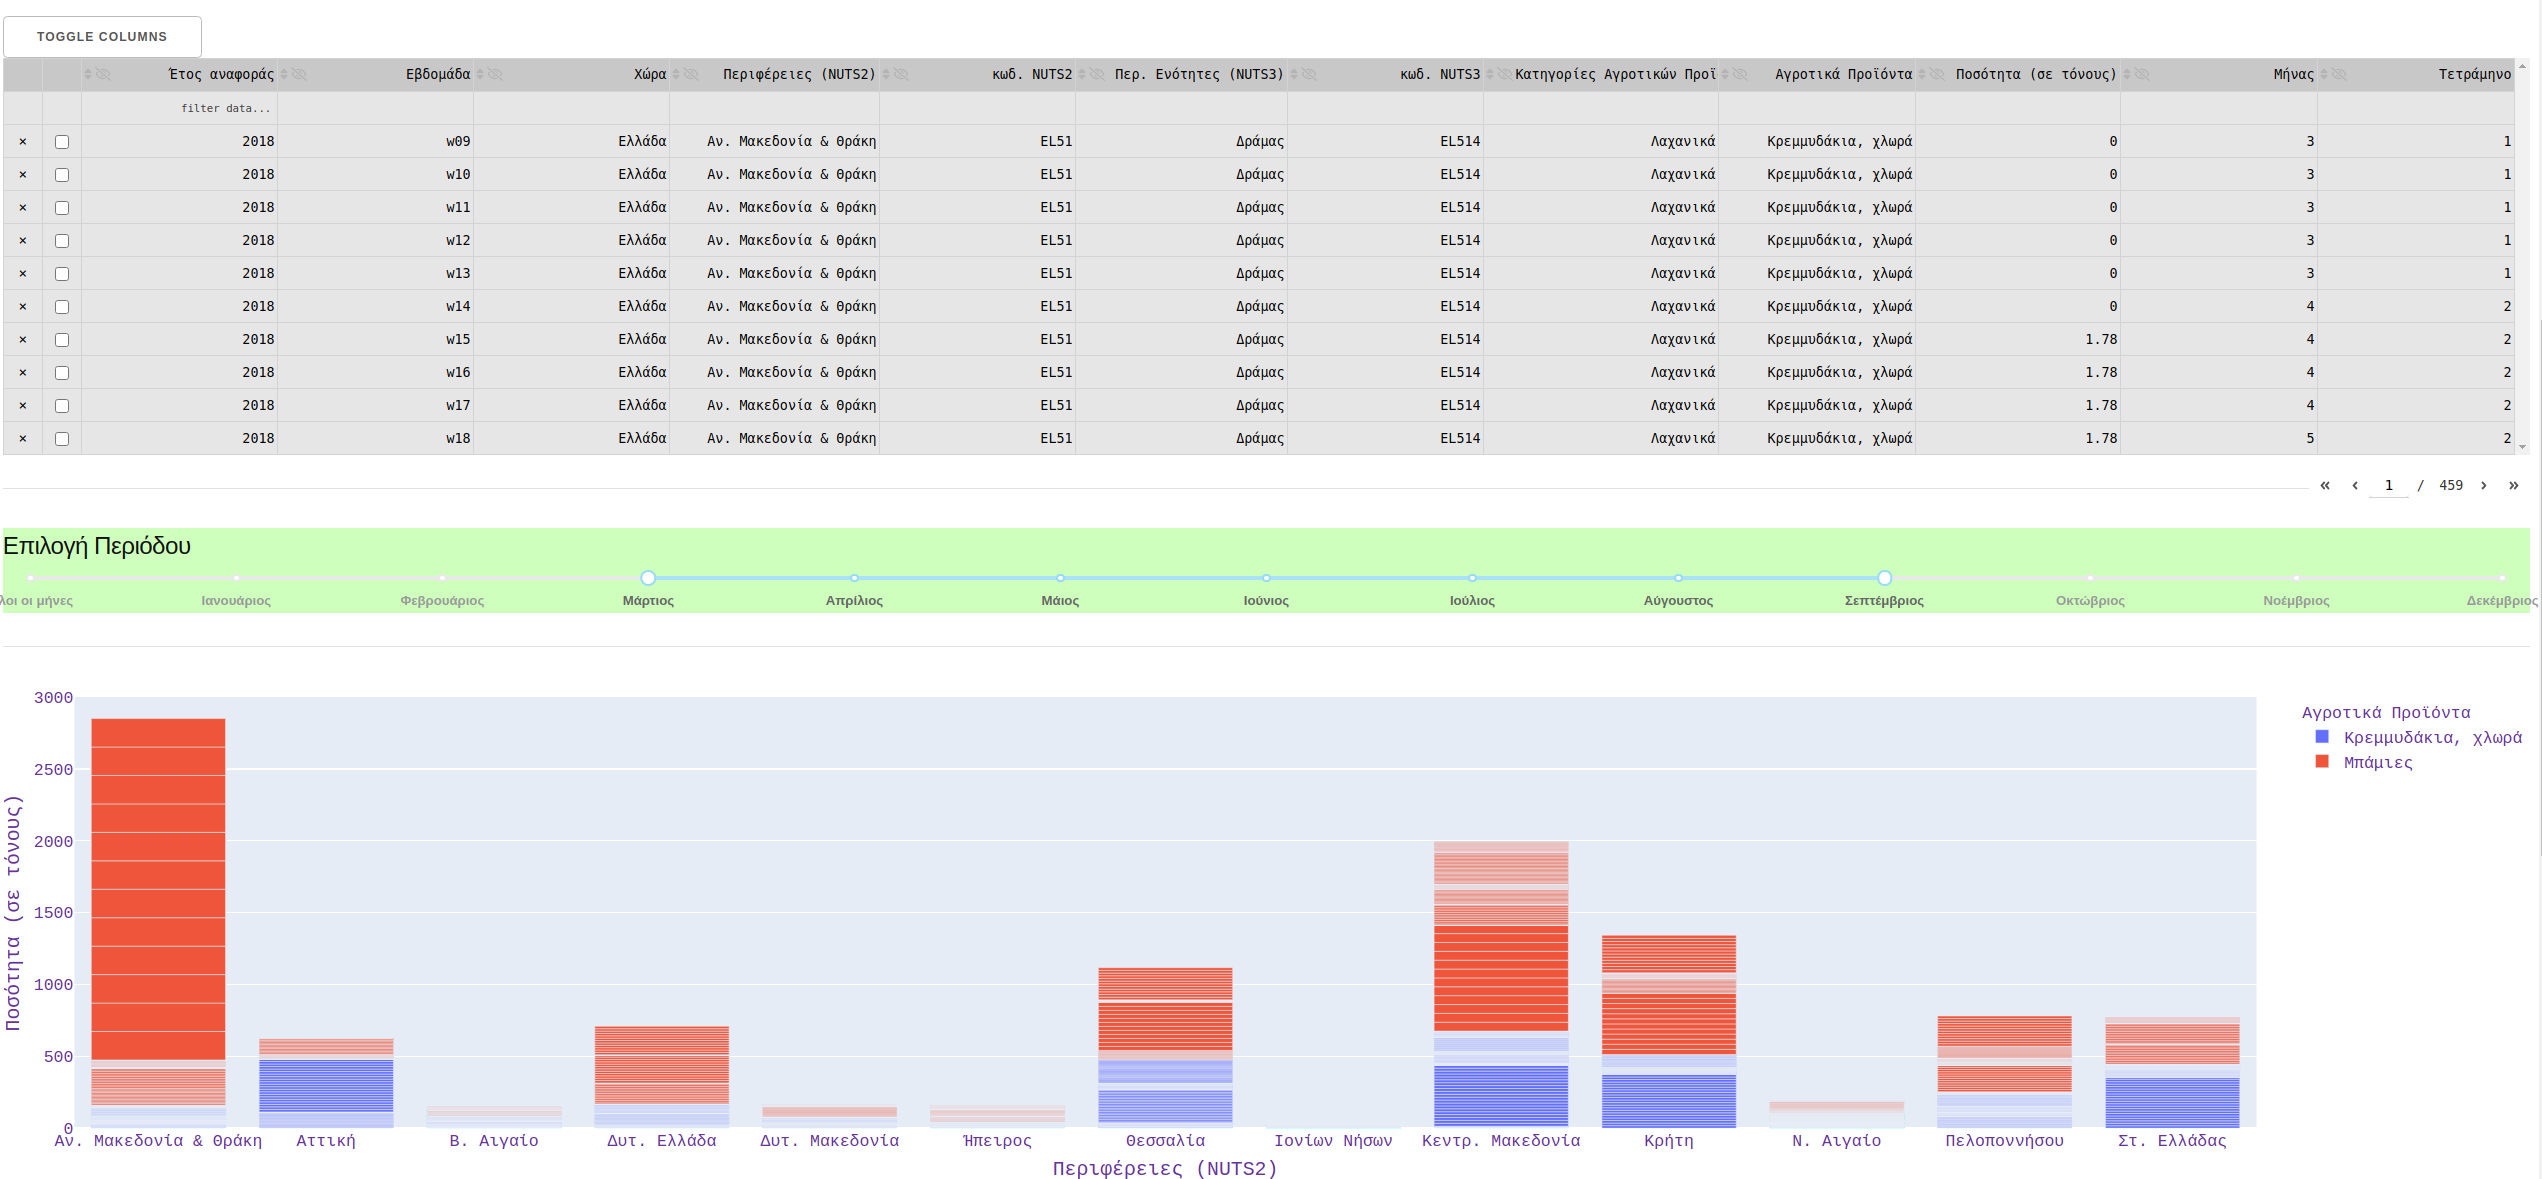
\includegraphics[width=3cm]{02_table_chart}
	%      \end{tabular}
	%
	%      \vspace{0.01em}
	%        \begin{tabular}{cc}
	%        example2  & example3 \\
	%        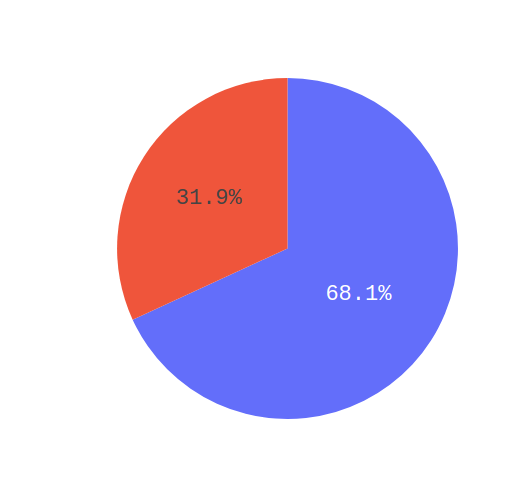
\includegraphics[width=3cm]{03_pie}
	%         &
	%         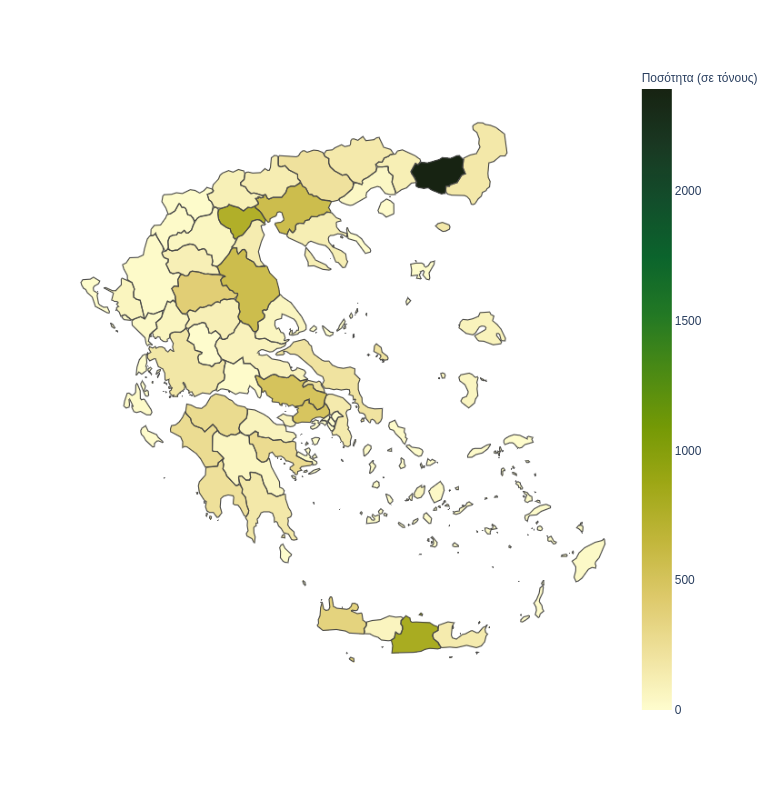
\includegraphics[width=3cm]{04_choropleth}
	%         \end{tabular}
		\begin{figure}[h]
		\begin{columns}[t]
			\column{.5\textwidth}
				\centering
				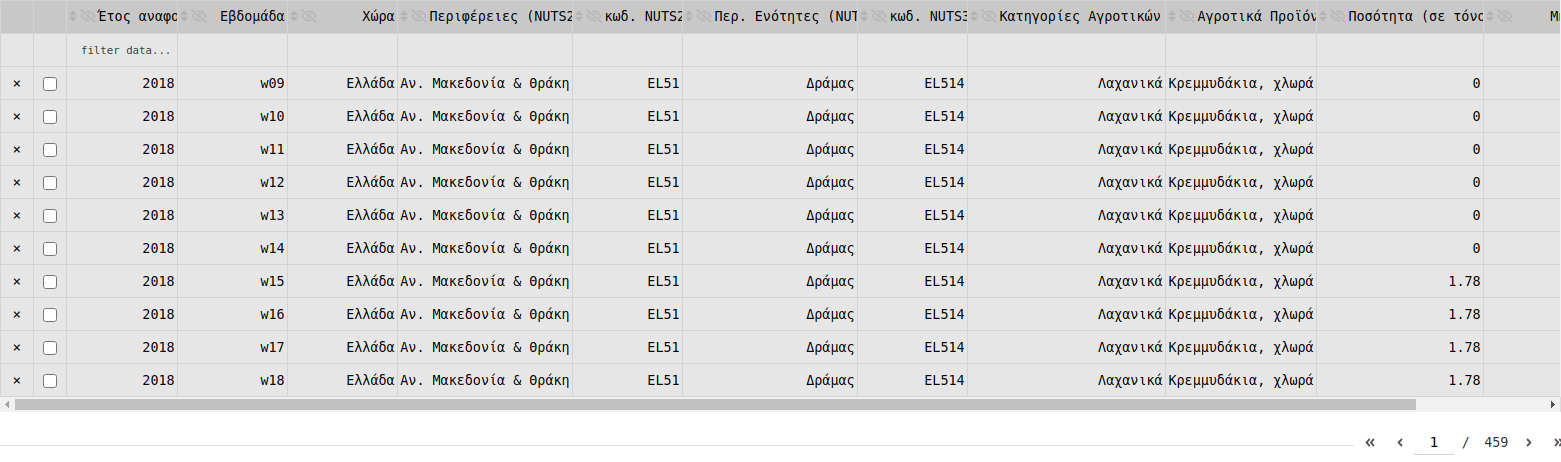
\includegraphics[width=5cm,height=2cm]{05_table}\\
				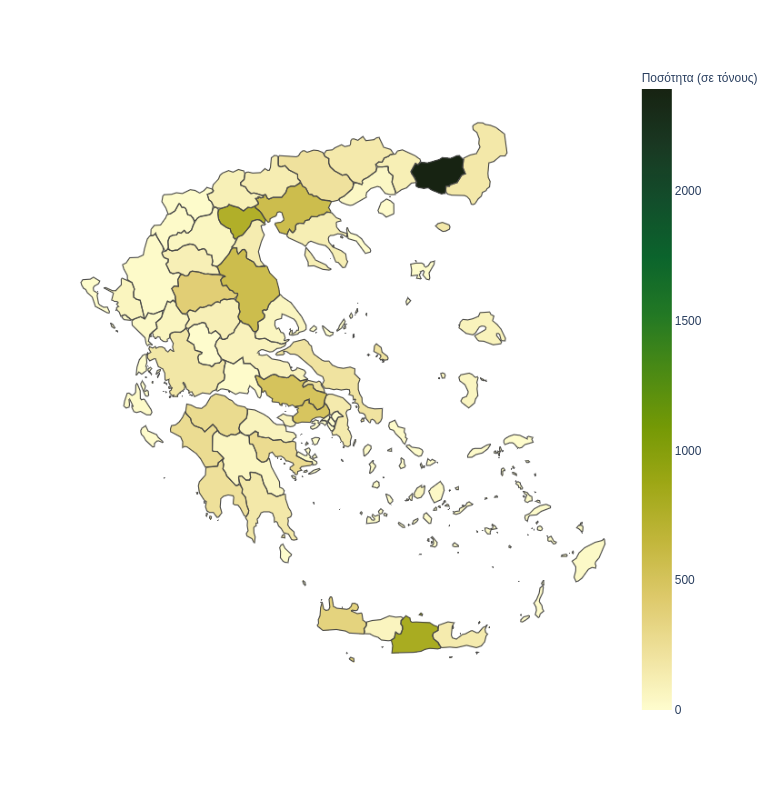
\includegraphics[width=3cm,height=2cm]{04_choropleth}
			\column{.5\textwidth}
				\centering
				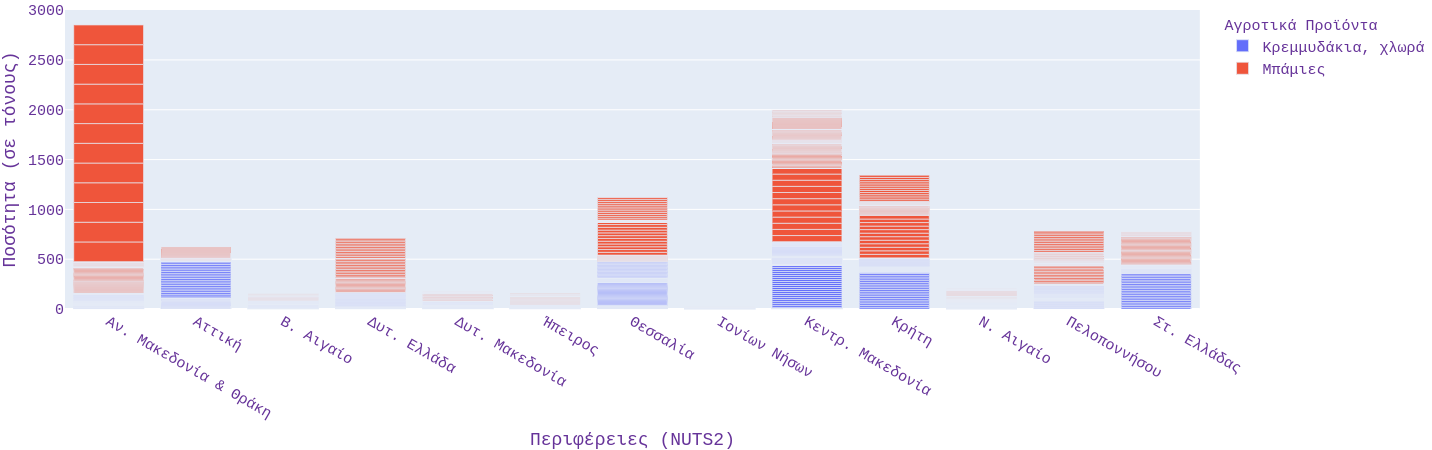
\includegraphics[width=5cm,height=2cm]{06_chart}\\
				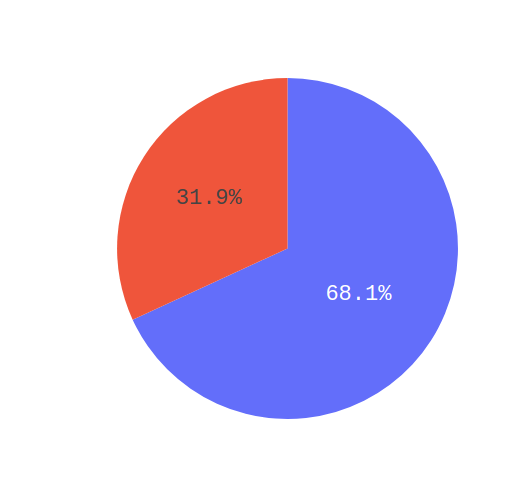
\includegraphics[width=2cm,height=2cm]{03_pie}
			\end{columns}
			\caption{Data visualization.}
			\label{fig:visuals}
	    \end{figure} 
    \end{frame}
    
    \begin{frame}
    \frametitle{Overview of platform basics}
    \checkmark A platform for data manipulation.\\
    \checkmark Integration of data of interest with geodata.\\
    \checkmark Visualization of combined data to maps.
    \pause
    \begin{alertblock}{Added value?}
    By selecting a custom data sub-set the user may further take advantage of the platform for valuable insights via a set of web-apps.
    \end{alertblock}
    \end{frame}
    
    \begin{frame}
    \frametitle{Applications on selected data: Four Step Model Example}
    With the selection of the dataset of interest the user may procceed to run a four step model on it.
    \begin{itemize}
    	\item The user may select the dataset of choice for the four step model execution.
    	\item The user may customize the four step model by selecting a friction function.
    \end{itemize}
    
    \begin{figure}[h]
    \centering
    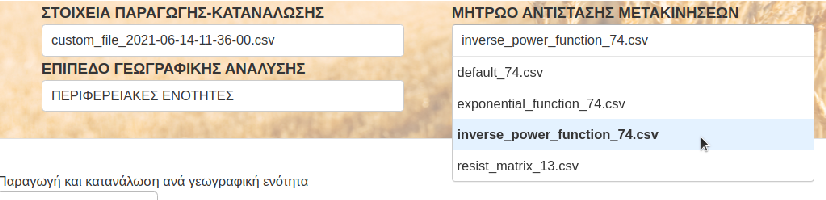
\includegraphics[width=8cm, height=2cm]{12_4sm_filters}
    \caption{Selection of custom dataset and friction function for the Four Step Model Execution.}
    \label{fig:4sm_filters}
    \end{figure}
    
    \end{frame}
    
    \begin{frame}
    
    \begin{exampleblock}{Four Step Model app execution}
    \frametitle{Applications on selected data: Four Step Model Example}
	    \checkmark Custom data set that used as input is presented.\\
	    \checkmark Origin-Destination Matrix with highlighted values is presented.
	\end{exampleblock}
	
	\begin{figure}[h]
    \centering
    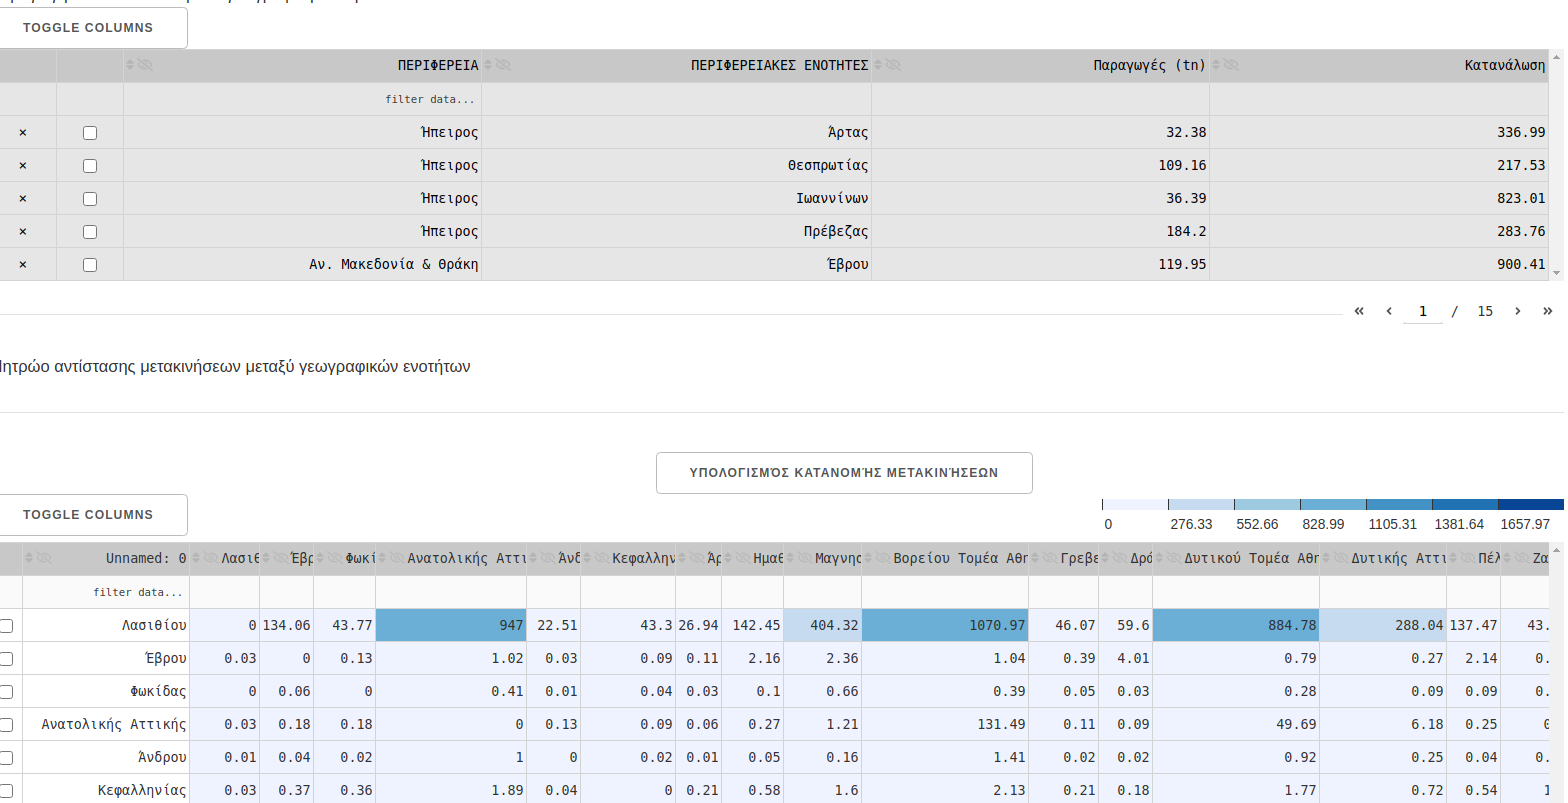
\includegraphics[width=8cm, height=3cm]{08_4sm}
    \caption{Four Step Model Execution based on user data selection.}
    \label{fig:4sm}
    \end{figure}
    
    \end{frame}

\section{Conclusions}

	\begin{frame}
    \frametitle{Conclusions - Added value}
    Platform created as Proof of Concept.
    \begin{itemize}
        \item A web-based transportation platform can be built solely on open tools and data.
        \item Such a platform is able to host applications and to implement functionality according to user requirements.
        \item A platform based on open data and tools is able to offer high-level solutions and customization.
        \item No proprietary software ensures sustainability of such a project.
    \end{itemize}
    
    \end{frame}
    
    \begin{frame}
    \frametitle{Restrictions - Future Work}
    \begin{itemize}
        \item Such a platform is heavily-bound to its users and the community.
        \item Challenge: Platform integration to open geodata ecosystem.
    \end{itemize}
    
    \end{frame}
    
    {
    \setbeamertemplate{footline}{\begin{tikzpicture}
    \node [inner sep=0pt, anchor=east] (0,0) {
\includegraphics[width=\paperwidth,height=0.8cm]{15_footnote_all}};
%    \node [inner sep=0pt, anchor=east] at (-2ex,-3ex) {\insertframenumber{} / %\inserttotalframenumber};
\end{tikzpicture}}
\placelogofalse
    \begin{frame}
    \frametitle{Thank you!}
    Thank you for your attention
    \end{frame}
}
	
\end{document}